\section{Testing Framework}
\label{sec:testing Framework}
Im folgenden Kapitel werden wir auf die einzelnen Komponenten des von uns entwickelten Test Frameworks eingehen und die Funktionsweise erläutern. Die Entwicklung des Test Framework wurde parallel zum RMIOnly- Systems mit Concurrency Control realisiert. Die Aufgabe des Test Framework liegt darin, die verschiedenen Prototypen, welche im Laufe dieser Semesterarbeit entwickelt wurden, mit Hilfe dieses Framework einheitlich testen zu lassen.


\subsection{Konzept}
Das Framework lässt sich über eine Konfigurationsdatei konfigurieren und kann Testfälle die in einer XML Datenstruktur vorliegen intepretieren und daraus die einzelnen Testszenarien generieren. Die Testszenarien werden vom Server auf die verfügbaren Testframework Clients verteilen und dort gestartet, hat ein Testframework Client ein Szenario auf einem ClientSystemUnderTest abgearbeitet, wird dieses zur Auswertung zurück an den Server geschickt. Auf dem Server werden die Messresultate jedes Szenario ausgewertet und abgespeichert. Dadurch lassen sich die Resultate der verschieden System zu einem späteren Zeitpunkt vergleichen.


\subsection{Server}
\label{sec:test-FW Server}
\begin{itemize}
\item Szenario definieren via XML (mit Beispiel?)
\item Konfiguration mit Property Datei
\item Resultate \& Auswertung
\item Vorbereitungs Task via Java RMI, Szenarien laden und verteilen
\item Für die Beweisführung das Lost Updates nicht mehr möglich sind, musste ein zusätzlicher Listener eingebaut der die event protokoliert.
\end{itemize}

\subsection{Testframework Client}
\label{sec:test-FW Client}
Diesem Kapitel beschreibt die Aufgaben des Testframework Client und deren Umsetzung. Der Framework Client lässt sich direkt vom Framework Server aus konfigurieren und steuern. Der Testframework Clients besitzt zwei Aufgaben, als erstes erzeugt und konfiguriert er das benötigte ClientSystemUnderTest. Zweitens muss er auf einem ClientSystemUnderTest eine gegebens Szenerio abarbeiten können. Die Realisierung des Testframeworks durch das bekannte Client/Server Konzepts führte zu eine schlanke Lösung und liesse sich jederzeit erweitern falls neue Anforderungen an das System gestellt werden.


\subsubsection{ClientController}
\label{sec:clientController}

\begin{center}
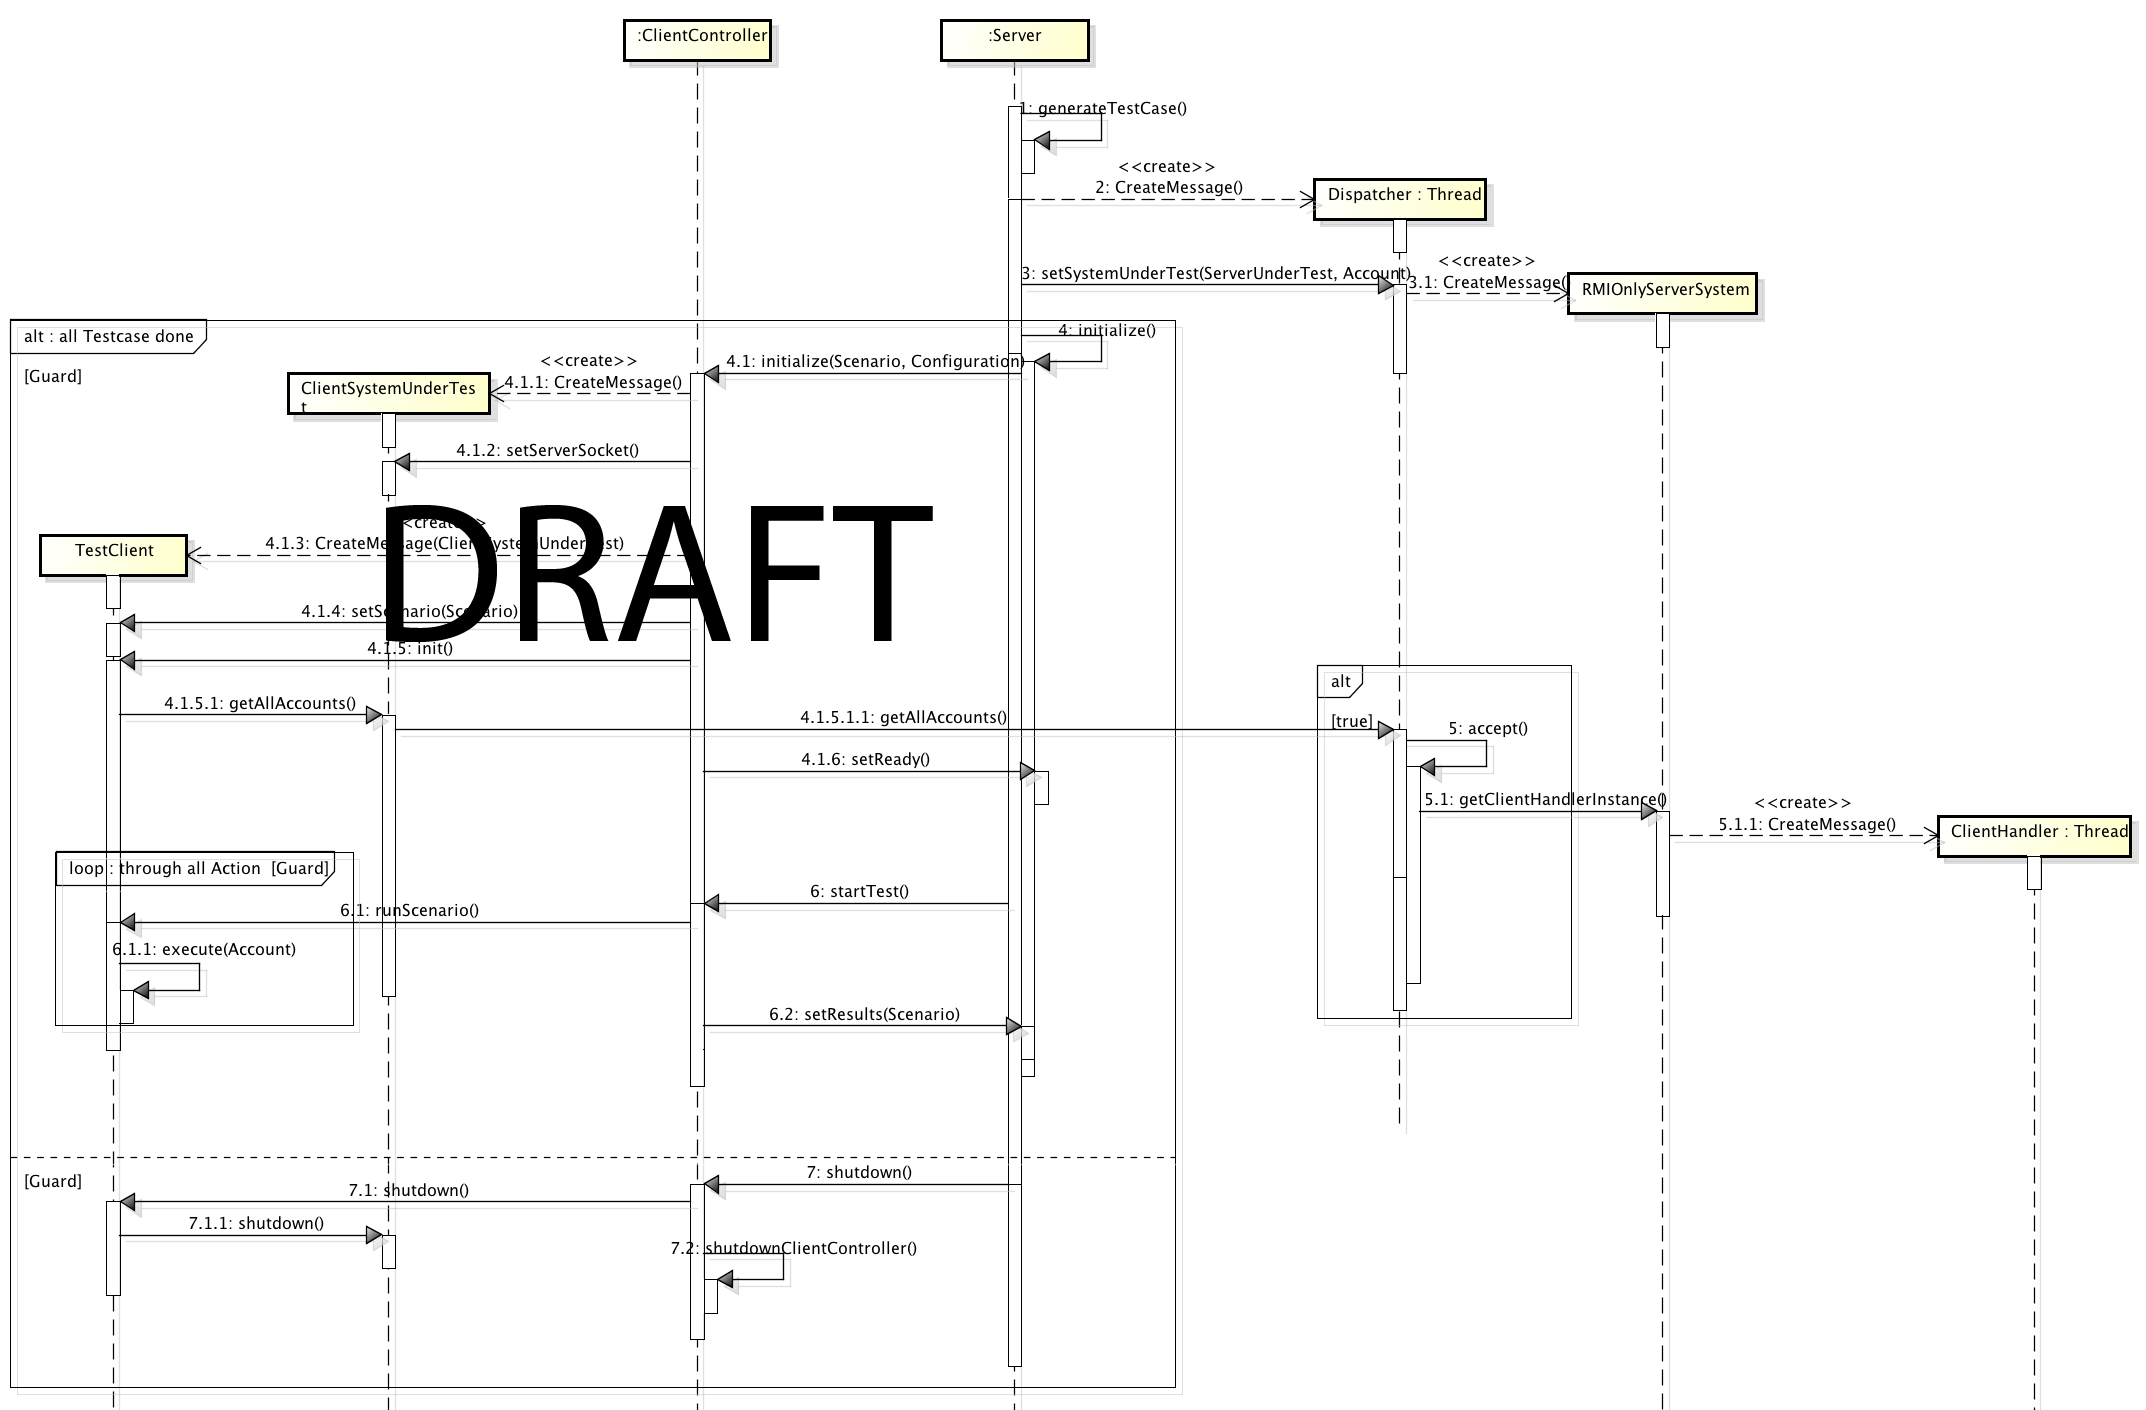
\includegraphics[scale=0.3]{image_testFramework/TestFWServerClientSeq.png}
\end{center}
 
Die Kommunikation zwischen den Testframework Clients und dem Server haben wir über Java RMI realisiert. Beim Start eines Testframework Clients wird ein ClientController instanziiert und diese wird dann zur Java RMI Runtime exportiert. Die veröffentlich das ClientController- Objekts erledigt die RMI Runtime im Hindergrund, ist das Objekt erfolgreich registriert, lässt es sich der Testframework Client über Remote Method Invocation vom Server kontrollieren. Es gibt zwei RMI Verbindungen, die eine vom Server zum Client, die zweite vom Client zurück zum Server. Der erste Kommunikationkanal wird für die Konfiguration und Steuerung des ClientController genutzt, die zweite Verbindung nutzt der ClientController für den Austausch von Resultate nach einem Testdurchlauf und für die Rückmeldung nach der Konfiguration eines ClientSystemUnderTest.

Folgendes Interface wird vom ClientController implementiert und lässt sich über RMI steuern:
\begin{lstlisting}	
public void initialize(Scenario scenario, Configuration configuration) throws RemoteException;
public void startTest() throws RemoteException;
public void shutdown() throws RemoteException;
\end{lstlisting}
Über dieses Interface lässt sich der gesamte Testprozess steuern. Zu Beginn wollten wir die Konfigurationswerte als Parameter übergeben, wir merkten jedoch schnell das es sinnvoller wäre einen Configuration Typ zu erstellen, der als reines Data Transfer Objekt dient und alle Parameter für die Konfiguration beinhaltet. Dieses Configuration beinhaltet underanderem den Namen des ClientSystemUnderTest sowie die nötigen Information für den erfolgreichen Aufbau der RMI Kommunikation zwischen dem Testframework Client und dem Testframework Server. In der initialize() Methode wird als erstes ein Server Stub geladen. Zweitens, wird aus dem Configuration Objekt das gewünschte ClientSystemUnderTest herausgelesen und via Reflection instanziiert. Danach wird ein neues TestClient-Objekt mit dem zuvor erzeugten CUT erzeugt. Als letztes wird der TestClient wird mit dem gegeben Szenario initialisiert. Sind alle Vorbereitungsschritte abgeschlossen, wird der Server über die erfolgreiche Initialisierung des CUT und des ClientController informiert. Der Server startet den Testdurchlauf parallel auf allen ClientController über die Methode startTest(). Sind alle Aktionen des gegeben Szenarios abgearbeitet, wird das gesamte Szenario mit den enthaltenen Messresultaten zurück an den Server geschickt, dort wird die Auswertung der Resultate vom Server erledigt. Der Testframework Client sowie das ClientSystemUnderTest laufen in derselben Java Virtual Machine um für jeden Testlauf dieselben JVM Umgebung zu gewährleisten, haben wir uns dazu entschlossen bei jedem Testcase das ganze System neu zu starten. Über die Methode shutdown() lässt sich der Testframework Client sowie der CUT herunterfahren.

\subsubsection{Test Client}
\label{sec:testclient}
Die Klasse TestClient ist die Schnittstelle zwischen dem Testframework und dem ClientSystemUnderTest. Im Konstruktor dieser Klasse kann ein Objekt übergeben werden, welches das ClientSystemUnderTest Interface implementiert. Startet der Server den Testlauf wird im TestClient das zuvor gesetzte Szenario abgearbeitet. Hierfür wird auf jedem Aktion Objekt die Methode execute(Account accunt) aufgerufen. Das Account Objekt, welches der execute Methode übergeben werden muss, wird aus der List von Accounts die von AccountService bereitgestellt wird geholt und übergeben.(Ringbuffer). Bei einem Shutdown durch den Server ist der TestClient ebenfalls für die beendigung des ClientSystemUnderTest zuständig.

\subsubsection{Action}
\label{sec:action}
Ein Szenario beinhaltet eine Menge von Aktionen die auf ein Account Objekt ausgeführt werden können. Für eine einfache Erweiterbarkeit von neuen Aktionen haben wir das Command-Pattern genutzt. Alle konkreten Implementierung von Aktionen leiten von der abstrakte Klasse Action ab. Diese abstrakte Klasse instanziiert im Konstruktor ein Result Objekt und deklariert drei Methoden die von Subklassen implementiert werden müssen. Das Result Objekt beinhaltet die alle Zeitmessungsdaten, die für diese Aktion gesammelt wurden. Bei der Ausführung des Scenarios nimmt der TestClient die Liste von Action aus dem Szenario und führt auf jeder Action execute() aus.
 
\subsubsection{Increment Action}
\label{sec:incrementAction}
Für unsere Anforderugen benötigten wir nur eine Aktion (Increment), die den aktuellen Kontostand des Account Objekts holt und den aktuellen Kontostand mit dem gegeben Faktor multipliziert und daraufhin den neuen berechneten Kontostand zurück in den Account schreibt. Zusätzlich war es nötig, dass zwischen der der getBalance() und der setBalance() eine definierbare Zeitdauer gewartet werden kann. Dies ist nötig damit sich leicht ein Konflikt erzeugen lässt und so gezeigt werden kann, dass dieser serverseitig zu keinem Lost-Updates führt. Tritt serverseitig ein Concurrency Fehler auf wird eine RuntimeExeption geworfen, die dazu führ das die ganze Aktion nochmals neugestartet wird mit dem Unterschied das diesmal keine Verzögerung zwischen getBalance() und setBalance() vorkommt.

\subsubsection{Result}
\label{sec:result}
Die Zeitmessung einer Aktion wir über den in Java eingebaute Zeitmessung Mechanismus System.nanoTime() aufgezeichnet. Die Result Klasse bietet eine startTimeMeasurement Methode die ein neues TimeRecord Objekt erzeugt und den momentane Zeitstempel in das TimeRecord Objekt schreibt, diese Methode verlangt eine BasicAction Typ der als Enum realisiert wurde(Erklärung warum nötig unter Resultate). Über stopTimeMeasurement() lässt sich die aktuelle Messung beenden und der aktuelle TimeRecord wird abgelegt. Da innerhalb der execute Methode mehrere setBalance() oder getBalance() möglich sind, müsste es möglich sein mehrere TimeRecords pro Result Objekt zuerfassen.




